\clearpage
\section*{\currfilename}

\begin{figure}[H]
  \fontsize{10pt}{10pt}\selectfont
  \begin{center}
    \begin{tikzpicture}[auto, scale=1.0, every node/.style={transform shape}, node distance=3cm,>=latex']
      \matrix[ampersand replacement=\&, row sep=1.0cm, node distance=3.0cm] (regions) at (0,0){
        \node [draw=black, label=below:{\shortstack[c]{GHV Equations\\ of Motion}}, label=above:{$A,B\Lambda,C$}, minimum width=2cm, inner sep=0mm] (R1){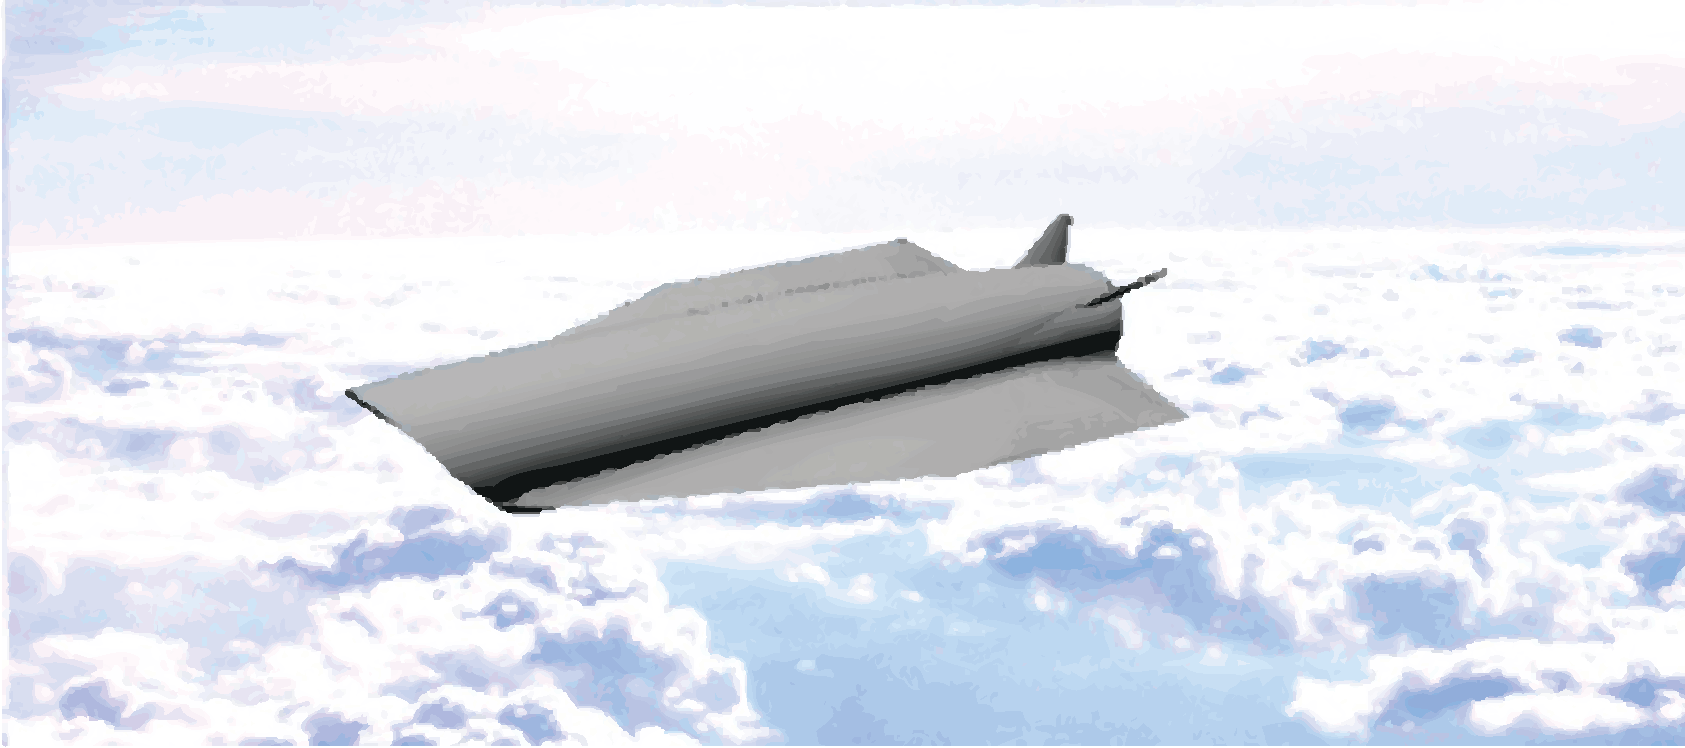
\includegraphics[width=4cm]{../fig/ghvclouds.pdf}}; \\
      };
      \matrix[ampersand replacement=\&, row sep=1.0cm, right of=R1, node distance=3.0cm] (R1out) {
        \node [whitesum] (R1outx) {}; \\
        \node [coordinate] (R1outP) {}; \\
      };
      \node[output, right of=R1outx,node distance=1.5cm](output1){};
      \node[output, below of=output1,node distance=1.0cm](output2){};
      \matrix[ampersand replacement=\&, row sep=0.6cm, left of=R1, node distance=4.0cm] (regions) {
        \node [block] (block2){\shortstack[c]{Adaptive\\ Controller}}; \\
      };
      \matrix[ampersand replacement=\&, row sep=0.6cm, left of=block2, node distance=3.0cm] (b2out) {
        \node [coordinate] (b2out1) {}; \\
        \node [coordinate] (b2out2) {}; \\
      };
      \node [coordinate, left of=b2out1, node distance=3.0cm] (input1) {};
      \node [coordinate, left of=b2out2, node distance=3.0cm] (input3) {};
      \node[input, above of=R1outx,node distance=1.0cm](input2){};
      \node[input, below of=block2,node distance=1.5cm](input4){};

      % Draw
      \draw [<-] (block2.west) + (0cm,0.3cm) -- node [near end]{$z_{\text{cmd}}$} (b2out1);
      \draw [<-] (block2.west) + (0cm,-0.3cm) -- node [near end]{$y$} (b2out2);
      \draw [->] (R1outx) -- node [pos=0.9]{} (output1);
      \draw [->] (block2) -- node [near start]{$u$} (R1);
      \draw [->] (input2) -- node [near start]{bias} (R1outx);
      \draw [->] (R1.east) + (0cm,0.5cm) -- (R1outx);
      \draw [->] (R1outx) -- node [pos=0.9]{} (output1);
      \draw [->] (R1.east) + (0cm,-0.5cm) -- node [pos=0.95]{$y$} (output2);
      %\draw [->] (input4) -- node [near start]{$S_{1}$, $L$} (block2);

      % Cross out
      \coordinate (arrow1) at ([xshift=-0.4cm,yshift=-0.3cm] output1);
      \coordinate (arrow2) at ([xshift=0.2cm,yshift=0.3cm] output1);
      \coordinate (arrow3) at ([xshift=-0.4cm,yshift=0.3cm] output1);
      \coordinate (arrow4) at ([xshift=0.2cm,yshift=-0.3cm] output1);
      \draw[-,red,line width=2](arrow1) -- (arrow2);
      \draw[-,red,line width=2](arrow3) -- (arrow4);
    \end{tikzpicture}
  \end{center}
\end{figure}
